\documentclass[letterpaper,10pt,onecolumn]{article}

\usepackage{setspace} 
\singlespacing
\usepackage{graphicx}                                        
\usepackage{amssymb}                                         
\usepackage{amsmath}                                         
\usepackage{amsthm}
\usepackage{mathtools}
\usepackage{algorithmic}
\usepackage{url}
\usepackage{tikz}         
\usetikzlibrary{matrix}
\usepackage{listings}
\usepackage{tabu}
\usepackage{mathptmx}
\usepackage{fullpage}
\usepackage{enumerate}
\usepackage{fancyvrb}
\usepackage{mathpartir}
\usepackage{lambda}
\usepackage{cc}
\usepackage{cc-ext}
                             

%%%
%%% Formatting details
%%%
\sloppy
\sloppypar
\widowpenalty=0
\clubpenalty=0
\displaywidowpenalty=0
\raggedbottom
\pagestyle{plain}

\DefineVerbatimEnvironment{program}{Verbatim}
  {baselinestretch=1.0,xleftmargin=5mm,fontsize=\small,samepage=true}

\def\denseitems{
    \itemsep1pt plus1pt minus1pt
    \parsep0pt plus0pt
    \parskip0pt\topsep0pt}

\newcommand{\tagtree}[3]{#1 \langle #2, #3 \rangle}

\usepackage{geometry}
\geometry{textheight=9.5in, textwidth=7in}
\parindent = 0.0 in
\parskip = 0.1 in
\title{Imperative Programming with Variational Effects}
\author{Alex Grasley}
\begin{document}

\maketitle

\section{Introduction}

%% TODO
Variation is a constant element in modern software systems. 

\section{Background}

\subsection{The choice calculus}

In order to formally represent choices in our programs we employ the choice
calculus \cite{ericthesis,erwig2011choice}. The fundamental unit of the choice calculus is
the \emph{choice}, which is a set of values called \emph{alternatives}.
There are many data structures that can be used to model
choices, but for our purposes we utilize a data structure we refer
to as a formula tree \cite{walkingshaw2014projectional,walkingshaw2014variational}.
Formula trees represent the set of alternatives as a binary tree, with concrete
values at the leaves of the tree. Each node of the tree is tagged with a formula from a boolean
algebra consisting of boolean literals, variables, negation, conjunction, and disjunction. We call individual
boolean variables the \emph{dimensions} of the choices, while the expressions as a whole we call \emph{conditions}. Notationally we represent these choice trees
via angle brackets. For example, a choice in dimension $A$
between the values $1$ and $2$ is written $\tagtree{A}{1}{2}$.

Each dimension can be viewed as coding for the presence or absence of a
particular feature that we wish to vary. To continue the above example, $\tagtree{A}{1}{2}$
represents a variational value that is $1$ when feature $A$ is present and $2$ otherwise. Conditions
are therefore analogous to conditional expressions built out of these features. For example, the choice $\tagtree{(A \wedge \neg B)}{1}{2}$
is a value that represents $1$ when feature $A$ is present and $B$ is absent, and $2$ otherwise.

The \emph{selection} operation on a choice can be used to eliminate conditions. We define a function
\emph{sel} that takes a \emph{selector} and a variational value and eliminates conditions based off
of the selector. For formula trees selectors are also booleans formulas, and can be seen as specifying
a condition that is assumed to hold true. Therefore, for a given condition and
selector, we eliminate the choice and replace it with the left branch if the selector logically implies
the truth of the condition. Similarly, if the selector logically implies the falsehood of the condition, we eliminate the choice
and replace it with the right branch. If neither implication is valid, the choice remains untouched with
both alternatives left intact.

It is often helpful to see this selection operation in action. The operation
$\mathit{sel}(A,\tagtree{A}{1}{2})$, can be seen as encoding the presence of feature $A$, which
will therefore produce the value $1$ as a result. Similarly, $\mathit{sel}(\neg A,\tagtree{A}{1}{2})$ can be seen as encoding the absence of feature $A$ and will
produce the value $2$. $\mathit{sel}(B,\tagtree{A}{1}{2})$ will result in an unchanged variational
value $\tagtree{A}{1}{2}$ because the selector $B$ does not logically imply either the truth or falsehood
of dimension $A$.

Selection is \emph{synchronized} for a given
condition, meaning that two choices in the same value or expression that share a condition must always
select the same alternative. For example, in the expression $\tagtree{A}{1}{2}+\tagtree{A}{3}{4}$,
the only possible selections are $1+3$ and $2+4$, while $1+4$ and $2+3$ can never occur due
to synchronization.

We say that a choice is \emph{configured} when all conditions
have been eliminated, yielding a plain value without choices. We call these resulting plain values
\emph{variants}. We define a function \emph{conf} which takes a
\emph{configuration} and a variational value and produces a variant. Under the view of dimensions as representing distinct features, a configuration for a formula tree gives
an assignment for each dimension of the variational value being configured.
A simple way to do this is to define a configuration as a list of the features that are present, with all
other features assumed to be absent. In other words, configurations are a list of variables that should
evaluate to true, with all other variables evaluating to false. Configuring a formula tree is then simply evaluating
each condition given the variable assignment. If the condition evaluates to true, then the left variant
is chosen, otherwise the right variant is chosen.

Using boolean formulas as our tags provides several advantages. For example, we can simplify trees like
$\tagtree{B}{1}{\tagtree{A}{1}{2}}$ to the more compact form $\tagtree{(B \vee A)}{1}{2}$. This is just
one of a number of optimizations that are made possible by representing tags as boolean formulas
\cite{walkingshaw2014projectional,hubbard2016formula}. Formula choices are also more convenient
for maintaining a variational context during execution of a program, a fact that will become
more relevant when we present our work on variational imperative programming later in
this work. Despite these advantages, formulas incur some cost by introducing boolean
satisfiability problems into many common operations, which is an NP-complete problem. However, thanks to improvements in the
efficiency of modern SAT solvers, often the worst-case NP-complete performance of these satisfiability
problems can be avoided.

\subsection{Implementation of Formula Trees}

When integrating formula trees into an existing non-variational language we can choose to
either embed choices directly into the abstract syntax of the host language or utilize a type-generic
implementation. In this work we employ both strategies, opting to embed choices directly when dealing
with programs, while using the type-generic implementation for the values produced by these programs.
Here we present the type-generic implementation, although the basic principles explored here apply
equally to embedded representations.

Generic formula trees can be represented by the following Haskell datatypes:

\begin{program}
type Dim = String
data Cond =
    Lit Bool
  | Ref Dim
  | Not Cond
  | And Cond Cond
  | Or Cond Cond

data V a = One a | Chc Cond (V a) (V a) 
\end{program}

The datatype \prog{Cond} represents expressions in our boolean algebra, with dimension names as strings.
The constructor \prog{One} creates the leaves of a formula tree, while \prog{Chc} creates the nodes.

This type-generic representation allows us to easily define some useful algebraic properties of
formula trees via typeclasses. Specifically, formula trees readily support implementation of the
Functor, Applicative, and Monad typeclasses:

\begin{program}
instance Functor V where
  fmap f (One a) = One (f a)
  fmap f (Chc d l r) = Chc d (fmap f l) (fmap f r)
  
instance Applicative V where
  pure = One
  (One f) <*> v = fmap f v
  (Chc d l r) <*> v = Chc d (l <*> v) (r <*> v)
  
instance Monad V where
  return = One
  (One v) >>= f = f v
  (Chc d l r) >>= f = Chc d (l >>= f) (r >>= f)
\end{program}

Astute readers will note that because formula trees are merely a special class of binary tree with
labeled nodes they share identical instances. The usefulness of defining these instances will be made
apparent further on in this work during the discussion of pure, side-effect free variational languages.

\subsection{Properties of choices}

% sharing is desirable. what is sharing?
The choice calculus gives us several desirable properties for variational programs.
The first is \emph{sharing}. A naive approach to executing a variational program is simply to
configure the variational program in order to produce each variant and run them all sequentially.
For a program with $n$ dimensions this results in $2^n$ variants that must be executed. Crucially,
the naive approach must recompute any common elements shared between variants. Embedding
choices in our program, combined with a variability-aware model of execution allows us to exploit this
inherent sharing by only computing shared components once, greatly improving the efficiency of
executing a variational program.

% correctness and the commuting diagram
Another property of choices and variation that we are interested in is \emph{correctness}. In order
to take advantage of the benefits of sharing, we must develop a variability-aware model of execution
that produces variational values as its result. In order to determine whether our variational results
are correct we need a way to relate them back to the individual variants they represent.

Given a function $f : T \rightarrow U$ and its variational counterpart $g : V \rightarrow W$, we say that
the relationship between the two is correct if for some configuration $c$ the following equality holds:
$\mathit{conf}\ c \circ g = f \circ \mathit{conf}\ c$ \cite{hubbard2016formula}. Put simply, configuring the result
of passing a variational value to a variational function should be the same as pre-configuring the input
and the function itself. This can be visualized as the following commuting diagram:

\begin{center}
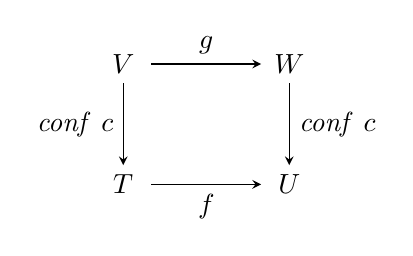
\begin{tikzpicture}
  \matrix (m) [matrix of math nodes,row sep=3em,column sep=4em,minimum width=2em]
  {
     V & W \\
     T & U \\};
  \path[-stealth]
    (m-1-1) edge node [left] {$\mathit{conf}\ c$} (m-2-1)
            edge node [above] {$g$} (m-1-2)
    (m-2-1.east|-m-2-2) edge node [below] {$f$}
             (m-2-2)
    (m-1-2) edge node [right] {$\mathit{conf}\ c$} (m-2-2)
            ;
\end{tikzpicture}
\end{center}

\section{Motivation}

In order to take advantage of the benefits of sharing provided by choices, we must develop variational
models of execution for a given language. We begin by showing that defining variational execution in a pure,
side-effect free evaluation context is a fairly straight-forward exercise before turning to the much more
difficult problem of variational execution with side effects.

\subsection{Pure variational execution}

If we do not have to worry about side effects in our language that we wish to introduce variation to then
our task is comparatively easy. We begin by considering a simple arithmetic expression language
defined by the following Haskell datatype:

\begin{program}
data Arith = N Int | Add Arith Arith | Mul Arith Arith
\end{program}

In the non-variational setting we can easily define an interpreter for this language which produces
values of type \prog{Int}:

\begin{program}
eval :: Arith -> Int
eval (N i) = i
eval (Add l r) = eval l + eval r
eval (Mul l r) = eval l * eval r
\end{program}

The process of ``variationalizing" this small example is quite straightforward. First, we add a
constructor to support choices in our language:

\begin{program}
data Arith = N Int | Add Arith Arith | Mul Arith Arith | AChc Cond Arith Arith
\end{program}

Next we modify our interpreter. Instead of returning plain values of type \prog{Int},
we now return \emph{variational} values of type \prog{V Int}. We then take the cases
from the non-variational interpreter and make them variational by situating them within the
applicative functor instance for \prog{V} we defined in Section 2. Finally, we add a case
that handles our new \prog{AChc} constructor and we have completed the conversion of our
interpreter:

\begin{program}
eval :: Arith -> V Int
eval (N i) = pure i
eval (Add l r) = (+) <$> eval l <*> eval r
eval (Mul l r) = (*) <$> eval l <*> eval r
eval (AChc d l r) = Chc d (eval l) (eval r)
\end{program}

This basic pattern of variationalizing a language by re-situating the
plain interpreter within the applicative functor for choices works well for any language that is pure
and side-effect free. The only area of concern is associated with the use of data structures in the
interpretation of the language, which often benefit from being replaced with custom variational data structures that
provide greater sharing and efficiency. Recent work has explored the benefits of custom variational
data structures for maps \cite{walkingshaw2014variational}, linked lists \cite{lists}, and stacks \cite{stacks}.
As such, exercising proper care in the selection and integration of variational data structures
into a variational interpreter resolves this issue.

Nevertheless, even with the support of more efficient
variational data structures, our basic pattern of converting a plain interpreter to a variational one
encounters significant difficulties in the presence of a language with side effects. Specifically, we
demonstrate that the presence of side-effectful statements, control flow structures, mutable state, and exceptions
commonly encountered in imperative programming languages requires more than the approach based
on applicative functors as we have outlined here.

\subsection{Mutable State}

To demonstrate why imperative programming with side effects requires us to rethink how we
variationalize a language and its execution, we turn to a small example in a simple imperative
language that supports basic control structures and variables with mutable state:

\begin{algorithmic}
\STATE $x \coloneqq 0$
\STATE $y \coloneqq$ getSecret()
\IF{$y$ is true}
\STATE{$x \coloneqq 1$}
\ENDIF
\end{algorithmic}

In a non-variational setting, we can reasonably expect the final state of the variables in this example
to be either $\{x \Rightarrow 0,\ y \Rightarrow \text{false}\}$ or
$\{x \Rightarrow 1,\ y \Rightarrow \text{true}\}$ depending on the value that
\prog{getSecret()} evaluates to. Now we consider the execution of the above example in a variational
setting. Suppose that the call to \prog{getSecret}
produces the variational value $\tagtree{A}{\text{true}}{\text{false}}$. We can view this as simply
combining the two possible non-variational execution paths described above into a
single execution varying in dimension $A$. As such, we would expect the final variable state
in this example to be  $\{x \Rightarrow \tagtree{A}{1}{0},\ y \Rightarrow \tagtree{A}{\text{true}}{\text{false}}\}$ by combining the final states above into choices over dimension $A$. We can verify this to be the proper variational result using the correctness relationship
specified in Section 2.

Of course, to arrive at the above result, we simply worked backwards from the non-variational
results. In order to take advantage of the benefits provided by sharing, we must instead develop a model
of variational execution that supports mutable state.  As we will see, the applicative functor instance for
\prog{V} is no longer sufficient by itself, necessitating a different approach to how we variationalize programs
that use mutable state.

The central problem becomes obvious when we compare the required semantic domains for evaluating statements
in the plain and variational versions of the example. The semantic domain of plain statements is a function from state to
state, where state is a mapping from variable names to values. As such, we might then assume that the corresponding
semantic domain for variational statements is also from state to state, only in this case we use a variational map. But when
we attempt to evaluate our example under this semantic domain we soon reach an issue that causes us to rethink our definition.

The problem comes in line 4, where we assign the variable $x$ in a conditional block. In the previous line, we check if the value of
$y$ is true. When $y$ is a variational value, allowing it to be both true or false in different variants, we only assign $x$ in those variants
in which $y$ is true. But if the state in our semantic domain is only a map, we have no way of passing the necessary information to the
assignment that it must only occur in particular variants and not in others. Our only choice is to assign the value of $x$ for all variants,
which would clearly be incorrect, as the assignment should only be carried out in the variant where $y$ is true. We must therefore
conclude that we need to carry this variational context information around in our state during execution in order to handle cases where
assignment occurs in a branch that is conditionally executed. Similar logic can be used to see that this context is also necessary to handle
variational lookup of variable values.

It is now clear why our previous approach of relying solely on the applicative functor instance for choices is inadequate. The method provides
no way of maintaining and manipulating variational context during execution. This nicely demonstrates the problems we encounter when
trying to introduce choices to languages with side effects.

%\begin{program}
%type Var = String
%data AExpr = N Int | Ref Var | GetSecret
%data BExpr = Equ AExpr AExpr
%data Stmt = Assn Var AExpr | If BExpr Block
%type Block = [Stmt]
%
%evalAExpr :: AExpr -> State -> Int
%evalAExpr (N i) _ = i
%evalAExpr (Ref x) s = lookup x s
%evalAExpr GetSecret = undefined
%
%evalBExpr :: BExpr -> State -> Bool
%evalBExpr (Equ l r) s = evalAExpr l s == evalAExpr r s
%
%evalStmt :: Stmt -> State -> State
%evalStmt (Assn x e) s = update x (evalAExpr e) s
%evalStmt (If e ss) s | evalBExpr e s = evalBlock ss s
%                     | otherwise     = s
% 
%evalBlock :: Block -> State -> State
%evalBlock b s = foldl (flip evalStmt) s b
%\end{program}

\subsection{Exceptions}

Exceptions are another common type of effect that proves challenging in a variational setting.
Consider the following program:

\begin{algorithmic}
\STATE $y \coloneqq$ getSecret()
\IF{$y$ is true}
\STATE{\textbf{throw} $e$}
\ENDIF
\STATE{$x \coloneqq$ expensiveFn()}
\end{algorithmic}

In a non-variational context, the behavior of this program should be clear.
If the variable $y$ evaluates to \textbf{true}, then an error is thrown with value
$e$. At this point evaluation should stop, meaning that the variable $x$ is never
assigned in the final statement, avoiding the costly computation of \prog{expensiveFn}. This effect of halting execution and
returning an error value is the essence of exceptions in non-variational settings.

Now we consider the behavior of the same program in a variational context.
Suppose that the variable $y$ evaluates to the variational value
$\tagtree{A}{true}{false}$. This means that in the left alternative of $A$ we
would evaluate the body of the if statement, while ignoring it otherwise. Therefore,
in the left alternative of $A$ we throw an exception, but otherwise we continue on to the
final statement.

Clearly maintaining the same behavior from the non-variational setting in the variational setting
violates correctness. If we halt execution whenever an exception is
thrown in any variant, then we also stop the evaluation of variants that never encountered an error,
as in our example for the case $\neg A$. Correctness dictates that variants that never encountered
an exception should complete their execution uninhibited.

We also can't simply continue evaluation
in every variant regardless of whether or not we have encountered an error.
Suppose that calling \texttt{expensiveFn} normally would evaluate to the variational value $\tagtree{A}{1}{2}$, but at considerable computational cost in both alternatives.
Because we know that the left alternative of $A$ will ultimately evaluate to the thrown exception $e$, we would
like to avoid the cost involved in computing the value $1$ that we will just throw away later, mirroring how throwing an exception short-circuits evaluation in the
non-variational setting. 

Another problem concerns how to keep track of which variants are in error states and what
the error values are. If we want to avoid the cost of pointless evaluation in variants that are in an error
state, we must have some efficient way of determining when evaluation is about to enter such a variant.
In the non-variational context we have no need to store and remember error values during evaluation
because we simply return the error value immediately when it is thrown. In the variational context, we
must now store these values while we continue to evaluate variants that are not in an error state.

\subsection{Comparison with Existing Work}

At this point, it should be apparent that introducing choices into a side-effectful imperative language
is anything but straightforward. The issues described above have been encountered repeatedly in efforts to
make variational versions of the While language \cite{varwhile}, PHP \cite{varex}, and Java \cite{varexj}.
The work on Varex the variational PHP interpreter, in particular demonstrates useful strategies for dealing
with mutable state and exceptions in a variational language.
In our work on the Resource DSL we independently discovered many of the same techniques used by Varex
to deal with these issues.
This work builds on the methods of handling variational effects discovered in the efforts to variationalize the
above languages by providing a formal operational semantics for the IMP language, a simple, albeit Turing-complete, imperative
language. It is our hope that a formal operational semantics for a simple imperative language will allow for easy application
and extension to variational imperative languages of differing levels of complexity.

\section{IMP with Effects}

\begin{figure}
\begin{syntax}
\text{(Arithmetic expressions)}\\
a &::=& n & \textit{Integer literal} \\
& | & x & \textit{Variable reference} \\
& | & a + a & \textit{Addition} \\
\text{(Boolean literals)} \\
b &::=& \CCkeyw{true} \\
& | & \CCkeyw{false} \\
\text{(Boolean expressions)} \\
e &::=& b & \textit{Boolean literal} \\
& | & \CCkeyw{not}\ e & \textit{Negation} \\
& | & e\ \CCkeyw{and}\ e & \textit{Conjunction} \\
& | & a < a & \textit{Less} \\
\text{(Statements)} \\
s &::=& \CCkeyw{skip} & \textit{Noop} \\
& | & x \coloneqq a & \textit{Assignment} \\
& | & s\ ;\ s & \textit{Sequencing} \\
& | & \CCkeyw{if}\ e\ \CCkeyw{then}\ s\ \CCkeyw{else}\ s & \textit{Conditional} \\
& | & \CCkeyw{while}\ e\ \CCkeyw{do}\ s & \textit{Looping} \\
& | & \CCkeyw{throw}\ a & \textit{Throw error} \\
& | & \CCkeyw{try}\ s\ \CCkeyw{catch}\ x\ \CCkeyw{in}\ s & \textit{Catch error}
\end{syntax}
\caption{Syntax of IMP with Effects}
\label{fig:impsyn}
\end{figure}

\def \BigN {\infer [A-Num] { } {(S,n) \Downarrow_A n}}

\def \BigVar {\infer [A-Ref] { } {(S,x) \Downarrow_A S(x)}}

\def \BigAdd {\infer [A-Add] {(S,a) \Downarrow_A n \\ (S,a') \Downarrow_A n' } {(S,a+a') \Downarrow_A n+n'}}

\def \BigB {\infer [B-Bool] { } {(S,b) \Downarrow_B b}}

\def \BigNot {\infer [B-Not] {(S,e) \Downarrow_B b} {(S,\CCkeyw{not}\ e) \Downarrow_B \neg b}}

\def \BigAnd {\infer [B-And] {(S,e) \Downarrow_B b \\ (S,e') \Downarrow_B b'} {(S,e\ \CCkeyw{and}\ e') \Downarrow_B b \wedge b'}}

\def \BigLess {\infer [B-Less] {(S,a) \Downarrow_A n \\ (S,a') \Downarrow_A n'} {(S,a<a') \Downarrow_B n<n'}}

\begin{figure}
\begin{syntax}
\text{(Store)}\\
S &::=& S(x) & \textit{Lookup x in S} \\
\end{syntax}

\begin{mathpar}
\BigN \and
\BigVar \and
\BigAdd \and
\BigB \and
\BigNot \and
\BigAnd \and
\BigLess
\end{mathpar}
\caption{Big-step semantics of IMP expressions}
\label{fig:impexpr}
\end{figure}

\def \nothing {\bullet}
\def \BigErr {\infer [S-Err] { } {(n,S,s) \Downarrow_S (n,S)}}
\def \BigSkip {\infer [S-Skip] { } {(E,S,\CCkeyw{skip}) \Downarrow_S (E,S)}}
\def \BigAssn {\infer [S-Assn] {(S,a) \Downarrow_A n} {(\nothing,S,x \coloneqq a) \Downarrow_S (\nothing,S[x \rightarrow n])}}
\def \BigSeq {\infer [S-Seq] {(E,S,s) \Downarrow_S (E',S') \\ (E',S',s') \Downarrow_S (E'',S'')} {(E,S,s\ ;\ s') \Downarrow_S (E'',S'')}}
\def \BigIfT {\infer [S-IfT] {(S,e) \Downarrow_B \CCkeyw{true} \\ (\nothing,S,s) \Downarrow_S (E,S')} {(\nothing,S,\CCkeyw{if}\ e\ \CCkeyw{then}\ s\ \CCkeyw{else}\ s') \Downarrow_S (E,S')}}
\def \BigIfF {\infer [S-IfF] {(S,e) \Downarrow_B \CCkeyw{false} \\ (\nothing,S,s') \Downarrow_S (E,S')} {(\nothing,S,\CCkeyw{if}\ e\ \CCkeyw{then}\ s\ \CCkeyw{else}\ s') \Downarrow_S (E,S')}}
\def \BigWhileT {\infer [S-WhileT] {(S,e) \Downarrow_B \CCkeyw{true} \\ (\nothing,S,s) \Downarrow_S (E,S') \\ (E,S',\CCkeyw{while}\ e\ \CCkeyw{do}\ s) \Downarrow_S (E',S'')} {(\nothing,S,\CCkeyw{while}\ e\ \CCkeyw{do}\ s) \Downarrow_S (E',S'')}}
\def \BigWhileF {\infer [S-WhileF] {(S,e) \Downarrow_B \CCkeyw{false}} {(E,S,\CCkeyw{while}\ e\ \CCkeyw{do}\ s) \Downarrow_S (E,S)}}
\def \BigThrow {\infer [S-Throw] {(S,a) \Downarrow_A n} {(\nothing,S,\CCkeyw{throw}\ a) \Downarrow_S (n,S)}}
\def \BigTry {\infer [S-Try] {(\nothing,S,s) \Downarrow_S (\nothing,S')} {(\nothing,S,\CCkeyw{try}\ s\ \CCkeyw{catch}\ x\ \CCkeyw{in}\ s') \Downarrow_S (\nothing,S')}}
\def \BigCatch {\infer [S-Catch] {(\nothing,S,s) \Downarrow_S (n,S') \\ (\nothing,S'[x \rightarrow n],s') \Downarrow_S (E,S'')} {(\nothing,S,\CCkeyw{try}\ s\ \CCkeyw{catch}\ x\ \CCkeyw{in}\ s') \Downarrow_S (E,S''[x \rightarrow S'(x)])}}

\begin{figure}
\begin{syntax}
\text{(Store)}\\
S &::=& S(x) & \textit{Lookup x in S} \\
& | & S[x \rightarrow n] & \textit{Update x in S to n} \\
\text{(Error context)} \\
E &::=& \nothing & \textit{No error} \\
& | & n & \textit{Error with value n}
\end{syntax}


\begin{mathpar}
\BigErr \and
\BigSkip \and
\BigAssn \and
\BigSeq \and
\BigIfT \and
\BigIfF \and
\BigWhileT \and
\BigWhileF \and
\BigThrow \and
\BigTry \and
\BigCatch
\end{mathpar}
\caption{Big-step semantics of IMP with Effects statements}
\label{fig:impstmt}
\end{figure}


\section{Variational IMP with Effects}

\begin{figure}
\begin{syntax}
\text{(Boolean literals)} \\
b &::=& \CCkeyw{true} \\
& | & \CCkeyw{false} \\
\text{(Conditions)}\\
C &::=& b & \textit{Boolean literal} \\
& | & D & \textit{Dimension name} \\
& | & \neg C & \textit{Negation} \\
& | & C \vee C & \textit{Disjunction} \\
& | & C \wedge C & \textit{Conjunction} \\
\text{(Arithmetic expressions)}\\
a &::=& n & \textit{Integer literal} \\
& | & x & \textit{Variable reference} \\
& | & a + a & \textit{Addition} \\
& | & \tagtree{C}{a}{a} & \textit{Choice} \\
\text{(Boolean expressions)} \\
e &::=& b & \textit{Boolean literal} \\
& | & \CCkeyw{not}\ e & \textit{Negation} \\
& | & e\ \CCkeyw{and}\ e & \textit{Conjunction} \\
& | & a < a & \textit{Less} \\
& | & \tagtree{C}{e}{e} & \textit{Choice} \\
\text{(Statements)} \\
s &::=& \CCkeyw{skip} & \textit{Noop} \\
& | & x \coloneqq a & \textit{Assignment} \\
& | & s\ ;\ s & \textit{Sequencing} \\
& | & \CCkeyw{if}\ e\ \CCkeyw{then}\ s\ \CCkeyw{else}\ s & \textit{Conditional} \\
& | & \CCkeyw{while}\ e\ \CCkeyw{do}\ s & \textit{Looping} \\
& | & \CCkeyw{throw}\ a & \textit{Throw error} \\
& | & \CCkeyw{try}\ s\ \CCkeyw{catch}\ x\ \CCkeyw{in}\ s & \textit{Catch error} \\
& | & \tagtree{C}{s}{s} & \textit{Choice}
\end{syntax}
\caption{Syntax of Variational IMP with Effects}
\label{fig:vimpsyn}
\end{figure}

\def \BigVNum {\infer [VA-Num] { } {(C,S,n) \Downarrow_{VA} n}}
\def \BigVRef {\infer [VA-Ref] { } {(C,S,x) \Downarrow_{VA} S(C,x)}}
\def \BigVAdd {\infer [VA-Add] {(C,S,e) \Downarrow_{VA} u \\ (C,S,e') \Downarrow_{VA} u'} {(C,S,e+e') \Downarrow_{VA} \mathit{liftA2}(+,u,u')}}
\def \BigVAChcOne {\infer [VA-Chc1] {\mathit{sat}(C \wedge C') \\ \mathit{sat}(C \wedge \neg C') \\ (C \wedge C',S,a) \Downarrow_{VA} u \\ (C \wedge \neg C',S,a') \Downarrow_{VA} u'} {(C,S,\tagtree{C'}{a}{a'}) \Downarrow_{VA} \tagtree{C'}{u}{u'}}}
\def \BigVAChcTwo {\infer [VA-Chc2] {\mathit{unsat}(C \wedge C') \\ \mathit{sat}(C \wedge \neg C') \\ (C \wedge \neg C',S,a') \Downarrow_{VA} u} {(C,S,\tagtree{A}{a}{a'}) \Downarrow_{VA} u}}
\def \BigVAChcThree {\infer [VA-Chc3] {\mathit{sat}(C \wedge C') \\ \mathit{unsat}(C \wedge \neg C') \\ (C \wedge C',S,a) \Downarrow_{VA} u} {(C,S,\tagtree{C'}{a}{a'}) \Downarrow_{VA} u}}

\def \BigVB {\infer [VB-Bool] { } {(C,S,b) \Downarrow_{VB} b}}
\def \BigVNot {\infer [VB-Not] {(C,S,e) \Downarrow_{VB} v} {(C,S,\CCkeyw{not}\ e) \Downarrow_{VB} \mathit{liftA}(\neg,v)}}
\def \BigVAnd {\infer [VB-And] {(C,S,e) \Downarrow_{VB} v \\ (C,S,e') \Downarrow_{VB} v'} {(C,S,e\ \CCkeyw{and}\ e') \Downarrow_{VB} \mathit{liftA2}(\wedge,v,v')}}
\def \BigVLess {\infer [VB-Less] {(C,S,e) \Downarrow_{VA} v \\ (C,S,e') \Downarrow_{VA} v'} {(C,S,e<e') \Downarrow_{VB} \mathit{liftA2}(<,v,v')}}
\def \BigVBChcOne {\infer [VB-Chc1] {\mathit{sat}(C \wedge C') \\ \mathit{sat}(C \wedge \neg C') \\ (C \wedge C',S,e) \Downarrow_{VB} v \\ (C \wedge \neg C',S,e') \Downarrow_{VB} v'} {(C,S,\tagtree{C'}{e}{e'}) \Downarrow_{VB} \tagtree{C'}{v}{v'}}}
\def \BigVBChcTwo {\infer [VB-Chc2] {\mathit{unsat}(C \wedge C') \\ \mathit{sat}(C \wedge \neg C') \\ (C \wedge \neg C',S,e') \Downarrow_{VB} v} {(C,S,\tagtree{C'}{e}{e'}) \Downarrow_{VB} v}}
\def \BigVBChcThree {\infer [VB-Chc3] {\mathit{sat}(C \wedge C') \\ \mathit{unsat}(C \wedge \neg C') \\ (C \wedge C',S,e) \Downarrow_{VB} v} {(C,S,\tagtree{C'}{e}{e'}) \Downarrow_{VB} v}}

\begin{figure}
\begin{syntax}
\text{(Store)}\\
S &::=& S(C,x) & \textit{Lookup x in S with context C} \\
\text{(Variational integers)}\\
u &::=& n & \textit{Integer literal} \\
& | & \tagtree{C}{u}{u} & \textit{Choice} \\
\text{(Variational booleans)}\\
v &::=& b & \textit{Boolean literal} \\
& | & \tagtree{C}{v}{v} & \textit{Choice}
\end{syntax}

\begin{mathpar}
\BigVNum \and
\BigVRef \and
\BigVAdd \and
\BigVAChcOne \and
\BigVAChcTwo \and
\BigVAChcThree \and
\BigVB \and
\BigVNot \and
\BigVAnd \and
\BigVLess \and
\BigVBChcOne \and
\BigVBChcTwo \and
\BigVBChcThree
\end{mathpar}
\label{fig:vimpexpr}
\caption{Big-step semantics of Variational IMP with Effects expressions}
\end{figure}

\newcommand{\GetCtx}[2]{\mathit{ctx}(#1,#2)}
\def \gc {\GetCtx{C}{E}}
\def \T {\mathit{true}}
\def \F {\mathit{false}}
\def \BigVUnsat {\infer [V-Unsat] {\mathit{unsat}(\gc)} {(C,S,E,s) \Downarrow_{V} (S,E)}}
\def \BigVSat {\infer [V-Sat] {\mathit{sat}(\gc) \\ (C,S,E,s) \Downarrow_{VS} (S',E')} {(C,S,E,s) \Downarrow_{V} (S',E')}}
\def \BigVSkip {\infer[VS-Skip] { } {(C,S,E,\CCkeyw{skip}) \Downarrow_{VS} (S,E)}}
\def \BigVAssn {\infer[VS-Assn] {(\gc,S,a) \Downarrow_{VA} u} {(C,S,E,x \coloneqq a) \Downarrow_{VS} (S[(\gc,x) \rightarrow u],E)}}
\def \BigVSeq {\infer [VS-Seq] {(C,S,E,s) \Downarrow_{V} (S',E') \\ (C',S',E',s') \Downarrow_{V} (S'',E'')} {(C,S,E,s\ ;\ s') \Downarrow_{VS} (S'',E'')}}
\def \BigVIf {\infer [VS-If] {(\gc,S,e) \Downarrow_{VB} v \\ (C \wedge \mathit{whenTrue}(v),S,E,s) \Downarrow_{V} (S',E') \\ (C \wedge \mathit{whenFalse}(v),S',E') \Downarrow_{V} (S'',E'')} {(C,S,E,\CCkeyw{if}\ e\ \CCkeyw{then}\ s\ \CCkeyw{else}\ s') \Downarrow_{VS} (S'',E'')}}
\def \BigVWhile {\infer [VS-While] {(\GetCtx{C}{E},S,e) \Downarrow_{VB} v \\ (C \wedge \mathit{whenTrue}(v),S,E,s) \Downarrow_{V} (S',E') \\ (C \wedge \mathit{whenTrue}(v),S',E',\CCkeyw{while}\ e\ \CCkeyw{do}\ s) \Downarrow_{V} (S'',E'')} {(C,S,E,\CCkeyw{while}\ e\ \CCkeyw{do}\ s) \Downarrow_{VS} (S'',E'')}}
\def \BigVThrow {\infer [VS-Throw] {(\GetCtx{C}{l:E},S,a) \Downarrow_{VA} u} {(C,S,l:E,\CCkeyw{throw}\ a) \Downarrow_{VS} (S,((C,u):l):E)}}
\def \BigVTry {\infer [VS-Try] {(C,S,[]:E,s) \Downarrow_{V} (S',[]:E)} {(C,S,E,\CCkeyw{try}\ s\ \CCkeyw{catch}\ x\ \CCkeyw{in}\ s') \Downarrow_{VS} (S',E)}}
\def \BigVCatch {\infer [VS-Catch] {(C,S,[]:E,s) \Downarrow_{V} (S',l:E) \\ (\GetCtx{C}{(l:[])},S'[(\GetCtx{C}{E},x) \rightarrow \mathit{combine}(l)],E,s') \Downarrow_{V} (S'',E')} {(C,S,E,\CCkeyw{try}\ s\ \CCkeyw{catch}\ x\ \CCkeyw{in}\ s') \Downarrow_{VS} (S''[(\T,x) \rightarrow S'(\T,x)],E')}}
\def \BigVChc {\infer [VS-Chc] {(C \wedge C',S,E,s) \Downarrow_{V} (S',E') \\ (C \wedge \neg C',S',E',s') \Downarrow_{V} (S'',E'')} {(C,S,E,\tagtree{C'}{s}{s'}) \Downarrow_{VS} (S'',E'')}}

\begin{figure}
\begin{syntax}
\text{(Store)}\\
S &::=& S(C,x) & \textit{Lookup x in S with context C} \\
& | & S[(C,x) \rightarrow u] & \textit{Update x in S to u with context C} \\
\text{(Variational integers)}\\
u &::=& n & \textit{Integer literal} \\
& | & \tagtree{C}{u}{u} & \textit{Choice} \\
\text{(Variational booleans)}\\
v &::=& b & \textit{Boolean literal} \\
& | & \tagtree{C}{v}{v} & \textit{Choice} \\
\text{(Error lists)} \\
l &::=& [] & \textit{Nil} \\
& | & (C,u):l & \textit{Cons} \\
\text{(Error context)} \\
E &::=& [] & \textit{Nil} \\
& | & l : E & \textit{Cons} \\ 
\end{syntax}


\begin{mathpar}
\BigVSat \and
\BigVUnsat \and
\BigVSkip \and
\BigVAssn \and
\BigVSeq \and
\BigVIf \and
\BigVWhile \and
\BigVThrow \and
\BigVTry \and
\BigVCatch \and
\BigVChc
\end{mathpar}
\caption{Big-step semantics of Variational Imp with Effects statements}
\label{fig:vimpstmt}
\end{figure}

\section{The Resource DSL}

The work on variational imperative programming we have described up to this point was motivated
by our experience developing the Resource DSL. The Resource DSL is designed with the intent of
allowing easy specification of resource requirements in highly configurable systems. Modern software
systems often have complex interactions in terms of resource requirements between different subsystems,
and managing these interactions and determining configurations that fulfill a certain set of requirements
is often a nontrivial task. The Resource DSL makes the specification and management
of these interactions much more feasible and maintainable. Because of the highly configurable and constantly evolving
nature of modern software systems the Resource DSL utilizes the principles of variational programming
discussed above in order to support the simultaneous verification of resource requirements for
systems with large feature sets. In this section we describe the design and implementation of the
Resource DSL including several case studies of its use. In particular we pay special attention to the
practical concerns brought on by integrating choices into an imperative language.

\subsection{Resources}

In our language a resource is represented by a distinct primitive value. These primitive values
can be either booleans, integers, floating point numbers, strings, or the unit value, as defined
by the following Haskell datatype:

\begin{program}
data PVal
     = Unit
     | B Bool
     | I Int
     | F Double
     | S Symbol
\end{program}

All resources are maintained in a global resource environment during execution of a program
in the Resource DSL. This environment is a mapping from paths to resource values. Paths are
analogous to the Unix filesystem paths that most programmers are already familiar with, allowing for
simple organization of resources in treelike structures. For example, a system may place its server
bandwidth resource at \prog{/Server/Bandwidth}, while placing its client bandwidth at \prog{/Client/Bandwidth}.
Again, by analogy to filesystem paths, resource paths can be either absolute or relative. Relative paths are
evaluated with respect to the execution environment's current path. For example, a reference to the resource
at the relative path \prog{../GPU/Speed} would evaluate to \prog{/Servers/Hardware/GPU/Speed}
given an execution environment with \prog{/Servers/Hardware/CPU} as its current path.

In a non-variational setting, resource environments could very easily be represented by a map data structure,
with paths as the keys and primitive values as the values. All interaction with the resource environment can then
simply be performed via the standard map operations (\emph{e.g.}, lookup, update, etc.). However, because our resource environment
is variational we must slightly tweak this implementation. Resources can have different values in different
variants, so we exchange values of type \prog{PVal} for \prog{V PVal}. But we soon note that simply exchanging primitive values
for choices of primitive values is insufficient, as we are unable to
account for cases where a resource is created or destroyed in only certain variants. We use \prog{Maybe} to represent this possibility
that a resource may only exist in certain variants, leaving us with \prog{V (Maybe PVal)} for the type of resources in the global environment.

Additionally, as explained in our discussion of the semantics of VIMP, all operations on our variational map must be variationally aware,
taking as an additional argument the current execution's variational context. The Resource DSL supports variationally aware lookup,
creation, deletion, and modification operations on variational maps. We provide a sample implementation of variational lookup, omitting
the other operations for brevity:

\begin{program}
vlookup :: (Ord k) => Cond -> k -> Map k (V (Maybe v)) -> V (Maybe v)
vlookup vctx k env = case (lookup k env) of
    Nothing -> One Nothing
    Just v -> sel vctx v  -- sel is the standard selection operation for formula trees
\end{program}

\subsection{Expressions}

Of course, primitive resource values are of little use without ways of manipulating them. To this end the Resource DSL supports
a number of common operations over primitive values in the form of a simple expression language. Expressions are formed by
immutable variable references, references to resources by their specific path, literal primitive values, and a number of common unary, binary, and ternary
operations, such as addition, negation, equality, ternary conditions, etc. Where appropriate, expressions utilize choices in order to support
variational execution.

\begin{program}
data Expr
     = Ref Var                             -- ^ variable reference
     | Res Path                            -- ^ resource reference
     | Lit (V PVal)                        -- ^ primitive literal
     | P1  Op1 (V Expr)                    -- ^ primitive unary function
     | P2  Op2 (V Expr) (V Expr)           -- ^ primitive binary function
     | P3 Op3 (V Expr) (V Expr) (V Expr) -- ^ conditional expression
\end{program}

The Resource DSL also supports unary functions over primitive values. The body of the function is simply a choice of expressions as defined above.
The function takes a single parameter, which is a combination of the name the parameter will be bound to in the body of the function and type of the parameter. Because the
type of the parameter may depend on the variant it is located in, we define types to be a choice of primitive types.

\begin{program}
data PType = TUnit | TBool | TInt | TFloat | TSymbol

data Param = Param Var (V PType)

data Fun = Fun Param (V Expr)
\end{program}

\subsection{Effects on Resources}

Having established the representation of resources in our DSL as well as their manipulation via expressions and unary functions,
we now turn to defining effects on the global resource environment.
The Resource DSL supports four basic effects for resources: creation, deletion, modification, and checking/verification. All effects are performed
within the current variational context of the execution. Deletion is the
simplest, removing the resource at a particular path. Creation takes a path and an expression that produces a variational primitive value
and inserts that value into the resource environment. Modification takes a unary function over the value of the resource and replaces it
with the result of the function. Checks take a unary function over the value of the resource that returns a boolean, with \prog{True} indicating
success and \prog{False} indicating failure. When a check fails, an error is thrown, with an error message indicating what check failed.
In this way, checks allow for a user to specify conditions or requirements that must hold for a particular resource.

\begin{program}
data Effect
     = Create (V Expr)
     | Check  Fun
     | Modify Fun
     | Delete
\end{program}

\subsection{Statements}

Statements are used in order to sequence and combine the above effects into programs in the Resource DSL.
The most basic statement is the \prog{Do} command, which takes a path to a resource and applies an effect to that
path. The other statements are a collection of control structures that allow for the sequencing and construction of
programs out of these \prog{Do} commands. \prog{If} and \prog{For} are straightforward control structures that allow
for conditional execution and looping, respectively. \prog{In} executes a block in the context of a particular path, where all
relative paths in an \prog{In} block are evaluated with reference to the supplied path value. This allows
users to easily describe work that should be done in particular resource sub-environments. \prog{Let} allows for the
extension of the current variable environment at the statement level. Finally, \prog{Load} permits the calling of named
subroutines with a list of arguments. 

One particular difficulty arises in determining how to represent a variational block of statements. Typically we
would use a simple list of statements, but in the variational setting we must ask what kind of variational list
we should use. Fortunately, recent work \cite{lists} has determined \emph{segment lists} to be a particularly
efficient implementation of variational linked lists. A segment list is a list of segments, where segments are either
plain lists or a choice between segment lists. Therefore, we define our blocks to be segment lists of
statements.

\begin{program}
data Segment a = Elems [a] | Split BExpr (SegList a) (SegList a)
type SegList a = [Segment a]
type Block = SegList Stmt

data Stmt
     = Do Path Effect
     | If (V Expr) Block Block
     | In Path Block
     | For Var (V Expr) Block
     | Let Var (V Expr) Block
     | Load (V Expr) [V Expr]
\end{program}


\bibliographystyle{plain}
\bibliography{paper}















\end{document}